% Data Source and Characteristics.
In this section, I describe the MUHC data warehouse (\gls{DW}) and how I plan to connect with it. A data warehouse is an enterprise data aggregation system which facilitates its collection, analysis, and reporting. The MUHC \gls{DW} is a newly created repository of clinical data connected to the hospital information system. It contains data on most process of care at the hospital and can be used for both quality improvement and research project. Data sources that are currently available include ADT, Medecho, Emergency Department, Medical Imaging, and the ICU registry while pharmacy data is scheduled for later integration. All sources are updated daily.

%The McGill University Health Centre Data Warehouse (MUHC DW) began in 2012 with an infrastructure   grant from the Canada Foundation for Innovation (CFI). Now, over 7.5 billion facts are accessible in 380 million rows, and over 6,000 columns, in 381 database tables. These data are linked together and organized for analyses of populations, with over 5.5 million health care episodes as of 2019, and is continually growing.

\begin{table}[h!]
\centering
\begin{tabular}{l|lllll}
\textbf{Year}       & 18   & 17   & 16   & 15   & 14   \\
\textbf{Patients}   & 1827 & 1739 & 1611 & 1535 & 1637 \\
\textbf{Physicians} & 265  & 269  & 266  & 278  & 278 
\end{tabular}
\caption{Counts of HF patients and their physicians, last 5 years, MUHC DW}
\end{table}

At this moment, no clinical data was obtained and I cannot present estimate for any potential clinical measure. However, a data dictionary is available describing the schema of the available data. I have received support from the director of the MUHC warehouse, Dr. David Buckeridge, for this project. A data request will be placed for any adult patient from the emergency department and intensive care unit identified by their ICD codes.\footnote{From "Get with the Guidelines - Heart Failure", from the American Heart Association}
% GWTG https://www.heart.org/idc/groups/heart-public/@wcm/@hcm/@gwtg/documents/downloadable/ucm_495599.pdf
Assigned to each patient, I will request the physician who signed the discharge, and their attending if present. Summary counts are presented in table 4.1. In case where both a resident and an attending are assigned to a patient, both will be considered responsible.

This project will use two datasets coming from the same source. A first, broader and denominalized, data request will be made for the purpose of finding targets in objective one and two. This request will be placed to the research pipeline of the data warehouse. At this point, unique anonymous IDs are sufficient. A second, precise, targeted, and nominalized data request will be made for the purpose of conducting the RCT. During this phase, I need to have the right provider see the right feedback, but these providers also need to see which patient might be in need of additional actions. All data collected by the systems will be linked to anonymous IDs.

All nominalized data will be kept in a remote secure server in the MUHC network. Feedback will also be created by the systems on this server. Anonymous data will be kept on a secure password protected computer, where the data analysis will also take place. All nominalized data will be removed as soon as the trial is over, while summary description of the anonymous data will be published along with the relevant research articles.

% Unsure about where to put in some graphical representation of the data I have here. Since the DW doesn,t have a good and nice visualization already built.

%\begin{wrapfigure}{r}{10cm}
  %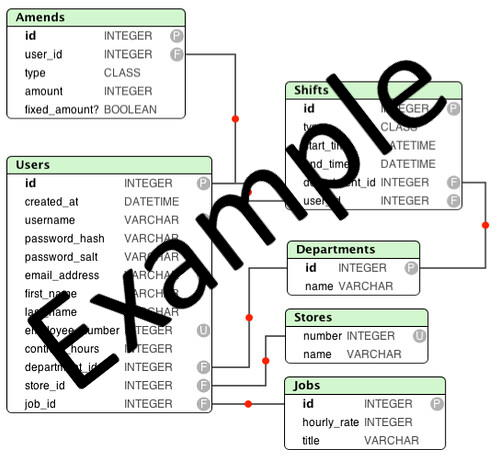
\includegraphics[width=\linewidth]{img/example_erd1.jpg}
  %\caption{Entities and their relationship in the data}
  %\label{fig:entity-relationship-diagram}
%\end{wrapfigure}